\chapter{Simulating Orbital Mechanics}
\section{Preface}
Text text text

\section{Relevant Physical and Mathetmatical Background}
\subsection{Classic Gravitational Force}
Already in the 17th century, \textit{Isaac Newton} formulated the gravitational force existing between any two objects with masses greater than zero. The strength of the force is given by the equation
\begin{equation}
    F = G\frac{m_{1}m_{2}}{r^{2}},
    \label{eq:force_gravity}
\end{equation}
where $m_{1}$ and $m_{2}$ are the respective masses of the two objects, $r$ is the distance between them, and $G$ is a the \textit{universal gravitational constant},
\begin{equation}
    G = \SI{6.6743(15)e-11}{\newton\metre\squared\per\kg\squared}
    \label{eq:universal_gravity_constant}
\end{equation}

The direction of the force is the line connecting the centers of mass of the two objects. Due to Newton's third law, the forces acting on the two objects are equal and opposite: the force applied by $m_{1}$ on $m_{2}$, $F_{1\to2}$, is pointing \textbf{from} $m_{2}$ \textbf{onto} $m_{1}$, and the force applied by $m_{2}$ on $m_{1}$, $F_{2\to1}$ is pointing \textbf{from} $m_{1}$ \textbf{onto} $m_{2}$ - and is exactly opposite to $F_{1\to2}$, i.e. in vector notation
\begin{equation}
    \vec{F}_{1\to2} = -\vec{F}_{2\to1}.
    \label{eq:gravity_force_vector_directions}
\end{equation}

If the two objects have positions $\vec{r}_{1}$ and $\vec{r}_{2}$, the vector pointing from object $1$ to object $2$ is
\begin{equation}
  \vec{r}_{1\to2} = \vec{r}_{2} - \vec{r}_{1},
  \label{eq:position_vector}
\end{equation}
with the vector pointing from object $2$ to object $1$ having the exact opposite components, i.e. $\vec{r}_{2\to1}=-\vec{r}_{1\to2}$. The norms of $\vec{r}_{1\to2}$ and $\vec{r}_{2\to1}$ are simply $r$ (the distance between the objects), and their directions are the unit vectors in the direction of $\vec{r}_{1\to2}$ and $\vec{r}_{2\to1}$, respectively:
\begin{align}
  \hat{r}_{1\to2} &= \frac{\vec{r}_{1\to2}}{\vnorm{r}_{1\to2}} = \frac{\vec{r}_{1\to2}}{r}\nonumber,\\
  \hat{r}_{2\to1} &= \frac{\vec{r}_{2\to1}}{\vnorm{r}_{2\to1}} = \frac{\vec{r}_{2\to1}}{r} = -\hat{r}_{1\to2}.
  \label{eq:normed_position_vector}
\end{align}

\begin{figure}
  \begin{center}
    \begin{tikzpicture}
      \pgfmathsetmacro{\a}{4}
      \pgfmathsetmacro{\b}{2}
      \coordinate (m1) at (0,0);
      \coordinate (m2) at (\a,\b);
      \coordinate (dp) at (-\b, \a);
      \coordinate (l1) at ($(m1)!1.3cm!(dp)$);
      \coordinate (l2) at ($(m2) + (m1)!1.3cm!(dp)$);
      \def\R{1cm}
      \def\r{0.5cm}
      \def\F{0.8cm}
      \draw[vector, xred, dashed] ($(m1)+(m1)!\R!(m2)$) -- ++($(m1)!\F!(m2)$) node[midway, below right, xshift=-1mm] {$\vec{F}_{2\to1}$};
      \draw[vector, xgreen, dashed] ($(m2)-(m1)!\r!(m2)$) -- ++($(m1)!-\F!(m2)$) node[midway, above left, xshift=1mm] {$\vec{F}_{1\to2}$};
      \draw[thick, fill=xgreen!50] (m1) circle (\R) node {$m_{1}$};
      \draw[thick, fill=xred!50] (m2) circle (\r) node {$m_{2}$};
      \draw[thick, cap=round, decorate, decoration={brace, amplitude=5pt}] (l1) -- (l2) node[midway, above left, xshift=0mm, yshift=2mm]{$r$};
      \draw[thick, densely dotted, black!75] ($(m1)+(m1)!0.15!(l1)$) -- (l1);
      \draw[thick, densely dotted, black!75] ($(m2)+(m1)!0.15!(l1)$) -- (l2);
    \end{tikzpicture}
  \end{center}
  \caption{Gravitational force between two objects with masses $m_{1}$ and $m_{2}$. Each object applies an attrctive force on the other object, with norm $F=G\frac{m_{1}m_{2}}{r^{2}}$ (where $r$ is the distance between the objects) and in the direction pointing from each object to the other object.}
  \label{fig:gravity_basics}
\end{figure}

In total, the vector notation of the gravitational force applied by the objects on each other are
\begin{align}
  \vec{F}_{1\to2} &= Gm_{1}m_{2}\frac{\hat{r}_{1\to2}}{r^{2}}\nonumber,\\
  \vec{F}_{2\to1} &= Gm_{1}m_{2}\frac{\hat{r}_{2\to1}}{r^{2}} = -\vec{F}_{1\to2}.
  \label{eq:gravity_forces_vector_notation}
\end{align}

\begin{note}{Another gravity force vector notation}{}
  In some textbooks, \autoref{eq:gravity_forces_vector_notation} are written without the unit vectors $\hat{r}_{1\to2}$ and $\hat{r}_{2\to1}$, instead using the distance vectors and dividing by $r^{3}$, i.e.
  \begin{align*}
    \vec{F}_{1\to2} &= Gm_{1}m_{2}\frac{\vec{r}_{1\to2}}{r^{3}},\\
    \vec{F}_{2\to1} &= Gm_{2}m_{1}\frac{\vec{r}_{2\to1}}{r^{3}}.
  \end{align*}
  The result is of course the same as in \autoref{eq:gravity_forces_vector_notation}, since for any non zero vector $\vec{v}$,
  \begin{align*}
    \frac{\vec{v}}{\vnorm{v}^{3}} = \frac{1}{\vnorm{v}^{2}}\frac{\vec{v}}{\vnorm{v}} = \frac{1}{\vnorm{v}^{2}}\hat{v}.
  \end{align*}
\end{note}

Let us look at an example of calculating the gravitational forces between two objects.

\begin{example}{Calculating a gravitational force}{grav_force_2_objects}
  Let us calculate the gravitational forces between two objects $A$ and $B$, using the following parameters:
  \begin{align*}
    \vec{r}_{A}&=\colvec{1;-2;0},\ m_{A} = 1,\\
    \vec{r}_{B}&=\colvec{2;5;-2},\ m_{B} = 2.
  \end{align*}
  For the sake of simplicity, we use $G=1$ and don't consider units with this example.

  The vector pointing from $A$ to $B$ is
  \[
    \vec{r}_{A\to B} = \vec{B}-\vec{A} = \colvec{2;5;-2} - \colvec{1;-2;0} = \colvec{1;7;-2},
  \]
  and the vector pointing from $B$ to $A$ is
  \[
    \vec{r}_{B\to A} = -\vec{r}_{A\to B} = \colvec{-1;-7;2}.
  \]

  The disntace $r$ between the objects is the norm of either of the above vectors, so we'll use $\vec{r}_{A\to B}$:
  \[
    r = \vnorm{r}_{A\to B} = \sqrt{1^{2}+7^{2}+2^{2}} = \sqrt{19} \approx 7.3485.
  \]

  The direction vectors are therefore
  \begin{align*}
    \hat{r}_{A\to B} &= \frac{1}{7.3485}\colvec{1;7;-2} = \colvec{0.1361;0.9526;-0.2722},\\
    \hat{r}_{B\to A} &= -\hat{r}_{A\to B} = \colvec{-0.1361;-0.9526;0.2722}.
  \end{align*}

  The gravity force which $A$ applies onto $B$ is then
  \[
    \vec{F}_{A\to B} = \cancel{G}\frac{\overbrace{m_{1}m_{2}}^{=2\times1}}{r^{2}}\hat{r}_{A\to B} = \frac{2}{54}\colvec{0.1361;0.9526;-0.2722} = \colvec{0.0050;0.0353;-0.101}.
  \]
  and similarily,
  \[
    \vec{F}_{B\to A} = -\vec{F}_{A\to B} = \colvec{-0.0050;-0.0353;0.101}.
  \]
\end{example}

In the case where we only consider two objects, and choose our frame of reference such that one of the objects is stationary - an analytical solution to the spatial trajectory taken by the second object is known and well studied. It is called a \textbf{Keplerian orbit}, and it always takes the form of a conic section.

\subsection{Conic Sections}
A conic section (sometimes simply just called \enquote{a conic}) is a 2-dimensional shape resulting from the intersection of a plane and a cone (see \autoref{fig:3d_conic_1}). Depending on the angle $\alpha$ by which the plane intersects the cone relative to the the cone's side, the resulting shape can be one of 3 general types (here $\theta$ is the cone's angle):
\begin{enumerate}
  \item If $\alpha>\theta$ the intersection is an \textbf{ellipse}. If in addition $\alpha=\ang{90}$ the ellipse becomes a \textbf{circle}.
  \item If $\alpha=\theta$ the intersection is a \textbf{parabola}.
  \item If $\alpha<\theta$ the intersection is a \textbf{hyperbola}.
\end{enumerate}

\begin{figure}
  \begin{center}
    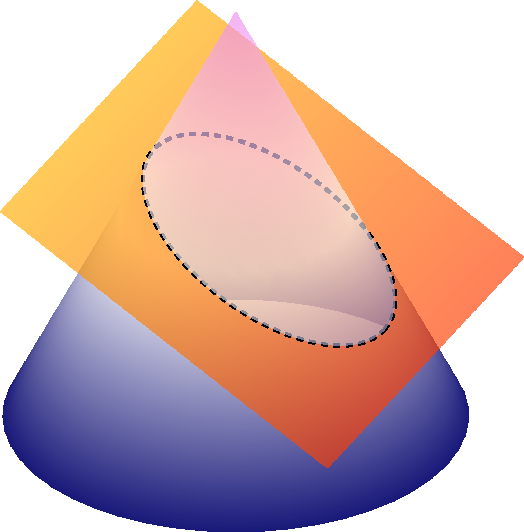
\includegraphics[scale=0.75]{figs/cone_plane_3d.pdf}
  \end{center}
  \caption{An intersection of a cone and a plane. Both the cone and plane are infinite - the cone extends infinitely \enquote{down}, but also has a second \enquote{inverted} part on the top, also extending to infinity. In the case here shown, the intersection is an ellipse. Image reproduced with modifications from !SOURCE!} % source: https://latexdraw.com/draw-a-plane-intersecting-a-cone-in-latex/
  \label{fig:3d_conic_1}
\end{figure}

\begin{figure}
  \begin{center}
    \begin{tikzpicture}
      \pgfmathsetmacro{\Lth}{1}
      \pgfmathsetmacro{\x}{2.25}
      \pgfmathsetmacro{\y}{3.5}
      \pgfmathsetmacro{\th}{atan(\y/\x)}
      \coordinate (h1) at (0,0);
      \coordinate (h2) at (0,-\y);

      % Cone
      \draw[filledangle={xpurple}] (h1) -- (0,-\Lth) arc (-90:-\th:\Lth) node [above, pos=0.37] {$\theta$};
      \draw[thick] (h1) -- (\x,-\y);
      \draw[thick] (h1) -- (-\x,-\y);
      \draw[thick, dashed, black!75] (-\x,-\y) -- ($(-\x,-\y)!1.4!(h1)$);
      \draw[thick] (-\x,-\y) -- ($(-\x,-\y)!1.2!(h1)$) node[above left, pos=0.6] {$C$};
      \draw[thick, dashed, black!75] (\x,-\y) -- ($(\x,-\y)!1.4!(h1)$);
      \draw[thick] (\x,-\y) -- ($(\x,-\y)!1.2!(h1)$);
      \draw[thick, dashed, black!75] (0,-\y) -- ($(0,-\y)!1.25!(h1)$) node[right, pos=0.05] {$h$};

      % Plane
      \pgfmathsetmacro{\px}{2}
      \pgfmathsetmacro{\pya}{1.25}
      \pgfmathsetmacro{\pyb}{2.25}
      \pgfmathsetmacro{\alph}{atan((\pyb-\pya)/(2*\px))}
      \pgfmathsetmacro{\Lalph}{0.75}
      \coordinate (p1) at (-\px,-\pya);
      \coordinate (p2) at (\px,-\pyb);
      \draw[thick, xred, dashed] (p1) -- ($(p1)!-0.2!(p2)$);
      \draw[thick, xred, dashed] (p2) -- ($(p1)!1.2!(p2)$);
      \draw[thick, xred, name path=p1--p2] (p1) -- (p2) node[above, pos=0.95] {$P$};
      \draw[name path=h1--h2, opacity=0] (h1) -- (h2);
      \path[name intersections={of=p1--p2 and h1--h2, by=E}];
      \draw[filledangle={xblue}] (E) -- ++(0,-\Lalph) arc (-90:-\alph:\Lalph) node[above, pos=0.35] {$\alpha$};
    \end{tikzpicture}
  \end{center}
  \caption{Side view of an infinite cone $C$ and an infinite plane $P$ intersecting it. The angle between $P$ and the cone's height line $h$ is $\alpha$, and the angle between the cone's surface and $h$ is $\theta$. In this figure $0<\theta<\alpha<\ang{90}$, and thus the shape formed by the intersection of $C$ and $P$ is an ellipse.}
  \label{fig:cone_side_view}
\end{figure}


\section{Forward Euler Method}

\section{Backward Euler Method}

\section{Verlet Integration}

\section{Runge-Kutta Method}
